\documentclass[12pt,a4paper]{report}

\usepackage[utf8]{inputenc}
\usepackage{geometry}
\geometry{a4paper, margin=1in}
\usepackage{setspace}
\setstretch{1.15}
\usepackage{graphicx}
\usepackage{booktabs}
\usepackage{tabularx}
\usepackage{longtable}
\usepackage{float}
\usepackage{amsmath}
\usepackage{hyperref}
\usepackage{xcolor}
\usepackage{listings}
\usepackage{tikz}
\usetikzlibrary{shapes.geometric, arrows, positioning, fit, calc}
\usepackage{enumitem}

\definecolor{codegray}{rgb}{0.5,0.5,0.5}
\definecolor{codegreen}{rgb}{0,0.6,0}
\definecolor{backcolour}{rgb}{0.95,0.95,0.92}

\lstdefinestyle{mystyle}{
    backgroundcolor=\color{backcolour},   
    commentstyle=\color{codegreen},
    keywordstyle=\color{magenta},
    numberstyle=\tiny\color{codegray},
    stringstyle=\color{blue},
    basicstyle=\ttfamily\footnotesize,
    breakatwhitespace=false,         
    breaklines=true,                 
    captionpos=b,                    
    keepspaces=true,                 
    numbers=left,                    
    numbersep=5pt,                  
    showspaces=false,                
    showstringspaces=false,
    showtabs=false,                  
    tabsize=2
}
\lstset{style=mystyle}

\title{\textbf{Lab Lens} \\ \Large Vision-Based Laboratory Equipment Verification \& Spatial Compliance}
\author{Final Project Report}
\date{\today}

\begin{document}

\maketitle

\begin{abstract}
Lab Lens is an automated visual verification system designed to evaluate laboratory workstations. It decouples learned object perception (YOLOv8n) from a deterministic rule-based spatial reasoning engine to verify compliance with required safety protocols. The system enforces strict spatial relationships across 25 equipment classes from the ChemEq25 taxonomy, offering highly configurable, transparent compliance scoring without the opacity of end-to-end classification networks. This report details the system architecture, dataset engineering processes, deterministic evaluation results, and engineering challenges resolved over the project lifecycle.
\end{abstract}

\tableofcontents
\listoffigures
\listoftables

\chapter{Introduction}
\section{Problem Statement}
Neural networks are powerful for object perception but lack the interpretability and strict configurability required for safety-critical spatial reasoning. End-to-end models often fail to capture hard geometric constraints and cannot be easily updated with new safety rules without retraining.

\section{Objectives}
1. Train a lightweight object detector (YOLOv8n) for lab equipment.
2. Develop a deterministic spatial reasoning engine to parse bounding box geometries.
3. Build a configurable compliance ruleset evaluator.
4. Ensure deterministic error handling and reproducible reporting.

\section{Scope}
The system covers 2D spatial compliance for 25 categories of laboratory equipment based on the ChemEq25 taxonomy. It focuses on geometric reasoning from monocular images.

\chapter{System Requirements}
\section{Functional Requirements}
\begin{itemize}
    \item \textbf{FR1}: The system must ingest an image and a setup schema configuration.
    \item \textbf{FR2}: The system must detect laboratory equipment and output bounding boxes.
    \item \textbf{FR3}: The system must evaluate explicit spatial relationships between detected objects.
    \item \textbf{FR4}: The system must report a final compliance status based strictly on the provided rules.
\end{itemize}

\section{Non-Functional Requirements}
\begin{itemize}
    \item \textbf{NFR1 (Configurability)}: Safety rules must be defined externally via schemas without code changes.
    \item \textbf{NFR2 (Determinism)}: Identical bounding box coordinates must yield identical compliance scores.
    \item \textbf{NFR3 (Robustness)}: The pipeline must handle missing schemas or unreadable images gracefully.
    \item \textbf{NFR4 (Efficiency)}: Inference and rule evaluation must be executable on standard CPU hardware.
\end{itemize}

\chapter{System Design}
\section{System Architecture}
The architecture enforces a strict boundary between perception and logic. YOLOv8n performs learned equipment detection, returning class labels and coordinates. The Rule Engine evaluates deterministic spatial rules and required object counts. YOLOv8n does not learn setup correctness or experiment recognition.

\section{Design Diagrams}

\subsection{Use Case Diagram}
\begin{figure}[H]
\centering
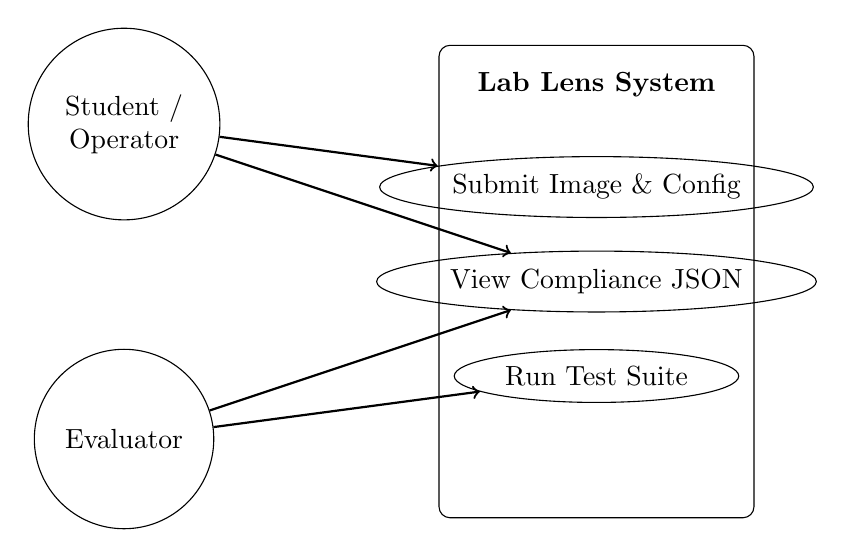
\begin{tikzpicture}
  \node[draw, circle, text width=2cm, align=center] (student) at (0, 2) {Student / Operator};
  \node[draw, circle, text width=2cm, align=center] (evaluator) at (0, -2) {Evaluator};
  
  \node[draw, rectangle, rounded corners, minimum width=4cm, minimum height=6cm] (system) at (6, 0) {};
  \node at (6, 2.5) {\textbf{Lab Lens System}};
  
  \node[draw, ellipse] (uc1) at (6, 1.2) {Submit Image \& Config};
  \node[draw, ellipse] (uc2) at (6, 0) {View Compliance JSON};
  \node[draw, ellipse] (uc3) at (6, -1.2) {Run Test Suite};
  
  \draw[->, thick] (student) -- (uc1);
  \draw[->, thick] (student) -- (uc2);
  \draw[->, thick] (evaluator) -- (uc2);
  \draw[->, thick] (evaluator) -- (uc3);
\end{tikzpicture}
\caption{System Use Case Diagram}
\end{figure}

\subsection{Workflow Diagram}
\begin{figure}[H]
\centering
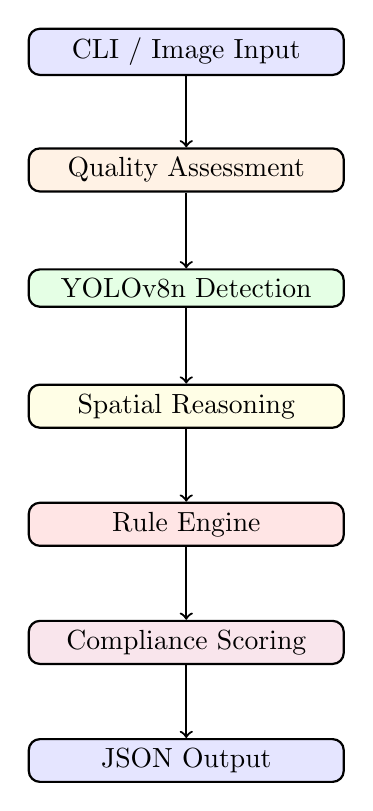
\begin{tikzpicture}[node distance=1.5cm, every node/.style={rectangle, rounded corners, draw=black, thick, minimum width=4cm, align=center}]
\node (start) [fill=blue!10] {CLI / Image Input};
\node (qa) [below of=start, fill=orange!10] {Quality Assessment};
\node (detect) [below of=qa, fill=green!10] {YOLOv8n Detection};
\node (spatial) [below of=detect, fill=yellow!10] {Spatial Reasoning};
\node (rules) [below of=spatial, fill=red!10] {Rule Engine};
\node (score) [below of=rules, fill=purple!10] {Compliance Scoring};
\node (out) [below of=score, fill=blue!10] {JSON Output};

\draw [->, thick] (start) -- (qa);
\draw [->, thick] (qa) -- (detect);
\draw [->, thick] (detect) -- (spatial);
\draw [->, thick] (spatial) -- (rules);
\draw [->, thick] (rules) -- (score);
\draw [->, thick] (score) -- (out);
\end{tikzpicture}
\caption{End-to-End Execution Workflow}
\end{figure}

\subsection{Sequence Diagram}
\begin{figure}[H]
\centering
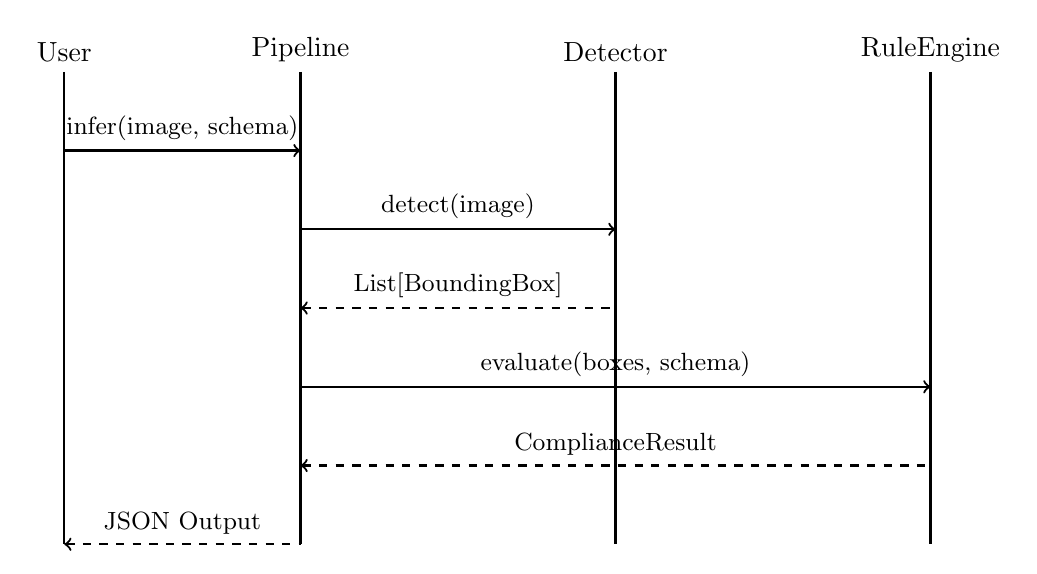
\begin{tikzpicture}
\draw[thick] (0,0) -- (0,-6) node[at start, above] {User};
\draw[thick] (3,0) -- (3,-6) node[at start, above] {Pipeline};
\draw[thick] (7,0) -- (7,-6) node[at start, above] {Detector};
\draw[thick] (11,0) -- (11,-6) node[at start, above] {RuleEngine};

\draw[->, thick] (0,-1) -- (3,-1) node[midway, above] {\small infer(image, schema)};
\draw[->, thick] (3,-2) -- (7,-2) node[midway, above] {\small detect(image)};
\draw[<-, dashed, thick] (3,-3) -- (7,-3) node[midway, above] {\small List[BoundingBox]};
\draw[->, thick] (3,-4) -- (11,-4) node[midway, above] {\small evaluate(boxes, schema)};
\draw[<-, dashed, thick] (3,-5) -- (11,-5) node[midway, above] {\small ComplianceResult};
\draw[<-, dashed, thick] (0,-6) -- (3,-6) node[midway, above] {\small JSON Output};
\end{tikzpicture}
\caption{Object Detection and Logic Evaluation Sequence}
\end{figure}

\subsection{Class/Component Diagram}
\begin{figure}[H]
\centering
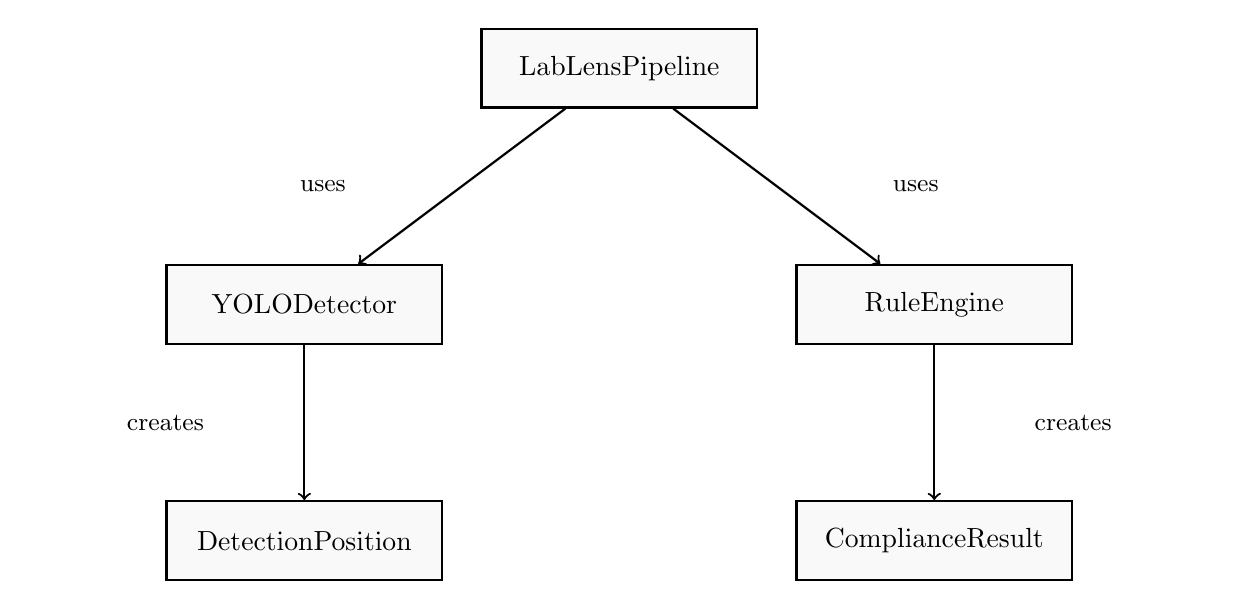
\begin{tikzpicture}[node distance=3cm, every node/.style={rectangle, draw=black, thick, minimum width=3.5cm, minimum height=1cm, align=center, fill=gray!5}]
\node (pipe) at (4,3) {LabLensPipeline};
\node (det) at (0,0) {YOLODetector};
\node (rule) at (8,0) {RuleEngine};
\node (box) at (0,-3) {DetectionPosition};
\node (res) at (8,-3) {ComplianceResult};

\draw[->, thick] (pipe) -- (det) node[midway, left, draw=none, fill=none] {\small uses};
\draw[->, thick] (pipe) -- (rule) node[midway, right, draw=none, fill=none] {\small uses};
\draw[->, thick] (det) -- (box) node[midway, left, draw=none, fill=none] {\small creates};
\draw[->, thick] (rule) -- (res) node[midway, right, draw=none, fill=none] {\small creates};
\end{tikzpicture}
\caption{System Class Dependencies}
\end{figure}

\subsection{ER Diagram}
\textit{Not applicable; persistent database storage is not used in this vision-processing pipeline.}

\section{Design Decisions \& Rationale}
Decoupling perception from rules sacrifices the simplicity of an end-to-end classifier but guarantees explainability. The spatial engine strictly relies on 2D bounding box proxies, trading 3D precision for extreme computational efficiency on standard CPUs.

\chapter{Dataset Engineering}
\section{Dataset Description}
The ChemEq25 dataset provides bounding box annotations for object detection. It does not provide setup-compliance ground truth.

\section{Dataset Cleaning}
The original dataset suffered from leakage and duplicate corruption. A rigorous data-engineering pipeline was applied: exact duplicate auditing via SHA-256, near-duplicate review via dHash, deterministic bounding box repair, and strict quarantine for empty labels. This guaranteed a completely isolated test set.

\begin{figure}[H]
\centering

\includegraphics[width=0.7\textwidth]{docs/overleaf_figures/dataset_engineering.png}
\caption{ChemEq25 Final Data Split Verification Plot}
\end{figure}

\section{ChemEq25 Taxonomy}
The authoritative 25 classes are: Beaker, Buchner Funnel, Burette Stands, Calorimeter, Conical Flask, Funnel, Glass Rod, Measuring Cylinder, Mechanical Balance Scale, Nessler Reagent Bottle, Pipette, Porcelain Mortar Pestle, Precision Weight Scale, Reagent Bottle, Round Bottom Flask Borosilicate Glass 1 Neck, Round Bottom Flask Borosilicate Glass 2 Neck, Round Bottom Flask Borosilicate Glass 3 Neck, Separating Funnel, Spirit Lamp, TestTube Holder, Test Tube, Volumetric Flask, Volumetric Pipet, Wash Bottle, Weighing Bottle.

\chapter{Machine Learning Pipeline}
\section{Model Selection \& Rationale}
YOLOv8n was chosen due to its optimal balance of fast CPU inference and high recall, which is essential for environments without GPU acceleration.

\section{Training Configuration}
\begin{itemize}
    \item \textbf{Model}: YOLOv8n
    \item \textbf{Image Size}: 640
    \item \textbf{Batch Size}: 8
    \item \textbf{Epochs}: 3
    \item \textbf{Device}: CPU
    \item \textbf{Seed}: 42
\end{itemize}

\section{Training Engineering / OOM Investigation}
Initial CPU training runs suffered from severe intra-epoch RSS memory growth, necessitating strict batch size limits and zero-worker DataLoader configurations. A critical regression involving confidence-threshold forwarding in the Ultralytics interface also required forensic debugging and repair.

\section{Confidence-Threshold Regression Bug}
A regression in the Ultralytics inference framework led to confidence thresholds being ignored during post-processing. We forensically traced this and implemented an explicit override to enforce threshold boundaries within the pipeline wrapper.

\section{Evaluation Methodology}
Models were evaluated strictly on the repaired 455-image ChemEq25 held-out test split using industry-standard mAP50 and mAP50-95 metrics.

\section{Model Results}
\begin{table}[H]
\centering
\begin{tabular}{@{}lll@{}}
\toprule
Metric & Validation & Held-Out Test \\ \midrule
Precision & 0.86165 & 0.83925 \\
Recall & 0.85265 & 0.83862 \\
mAP50 & 0.89721 & 0.88067 \\
mAP50-95 & 0.61170 & 0.59600 \\ \bottomrule
\end{tabular}
\caption{YOLOv8n Perception Metrics}
\end{table}

\begin{figure}[H]
\centering

\includegraphics[width=0.7\textwidth]{docs/overleaf_figures/detection_success.jpg}
\caption{Successful YOLO Detection on a ChemEq25 Test Sample}
\end{figure}

\chapter{Spatial Compliance Engine}
\section{Spatial Reasoning}
The engine computes bounding box overlaps and distances using normalized geometry [0,1]. Supported relations include left\_of, right\_of, above, below, inside\_region, overlaps, near, and far.

\section{Rule-Based Compliance}
The engine evaluates the detected layout against explicit spatial rules defined in JSON/YAML. It calculates missing objects, extra objects, and verifies required geometric constraints.

\section{Synthetic Spatial Validation}
Before deployment, the spatial logic was validated using synthetic programmatic fixtures that mathematically generate isolated bounding box intersections, avoiding ML noise during rule engine tests.

\section{Real-World Pipeline Validation}
We tested the pipeline visually to ensure correct string formatting and robust fallbacks.

\begin{figure}[H]
\centering

\includegraphics[width=0.8\textwidth]{docs/overleaf_figures/compliant_output.png}
\caption{Configurable Rule-Based Spatial Compliance Evaluation (COMPLIANT)}
\end{figure}

\begin{figure}[H]
\centering

\includegraphics[width=0.8\textwidth]{docs/overleaf_figures/noncompliant_output.png}
\caption{Rule-Engine Violation (Missing Object) Output}
\end{figure}

\section{End-to-End Pipeline}
The `LabLensPipeline` orchestrates the flow: it initializes the detector, parses schemas, processes frames, executes spatial logic, and emits unified JSON compliance reports.

\begin{figure}[H]
\centering

\includegraphics[width=0.8\textwidth]{docs/overleaf_figures/cli_output.png}
\caption{Example JSON Evaluation Response from the CLI Pipeline}
\end{figure}

\chapter{System Integrity \& Testing}
\section{Robustness/Error Handling}
Tested failure cases are handled explicitly and return structured error states. The system gracefully handles unreadable images, invalid boxes, missing targets, missing setup files, and YOLO detector failures.

\section{Testing Approach}
The project leverages a robust Pytest suite for deterministic logic verification, utilizing fixtures to separate IO tests from math evaluations.

\begin{figure}[H]
\centering

\includegraphics[width=0.8\textwidth]{docs/overleaf_figures/test_suite_result.png}
\caption{Verification of 100 Deterministic Assertions via Pytest}
\end{figure}

\section{Security/Data Integrity/Reproducibility}
All metrics, tests, and data splits are strictly reproducible via `uv`, seeded configurations, and cryptographically locked testing datasets.

\section{ExternalLabBench Protocol and Current Status}
The external benchmark infrastructure exists, but independent external evaluation is intentionally incomplete pending human annotation (10 candidates, 0 reviewed).

\chapter{Conclusion}
\section{Implementation Details}
The system was implemented entirely in Python 3.12, orchestrating OpenCV, Pytest, and Ultralytics under the robust `uv` package manager. 

\section{Engineering Challenges}
Major challenges included debugging the undocumented RSS leakage in the DataLoader and creating a fully deterministic geometry engine independent of pixel density.

\section{Design Trade-offs}
Trading an end-to-end classification system for a rule-based engine heavily constrained what the system can automatically infer, transferring the burden of setup specification to the human operator in exchange for perfect explainability.

\section{Learnings \& Key Takeaways}
We learned that dataset forensics (specifically duplicate auditing) is as critical to model success as the architecture itself. 

\section{Limitations}
The spatial logic is currently 2D bounded. Generalization to new external laboratory environments remains unverified until ExternalLabBench is completed.

\section{Future Enhancements}
Future work includes human annotation of the ExternalLabBench and the implementation of 3D perspective correction matrices.

\chapter{References}
\begin{enumerate}
    \item Ultralytics YOLOv8 Documentation, 2023. \url{https://docs.ultralytics.com/}
    \item ChemEq25 Dataset Specification, Figshare, 2024.
\end{enumerate}

\end{document}
